\section{Language}
\label{sec:language}

% present ndlog first as in sigcomm paper
% talk about events, etc extensions for soft-state

In this section we present an overview of the Network Datalog
(\Dlog) language for declarative networking. The \Dlog language is
based on extensions to traditional Datalog, a well-known recursive
query language designed for querying graph-structured
data in a centralized database. \Dlog's integration of networking and
logic is unique from the perspectives of both domains.  As a network
protocol language, it is notable for the absence of any communication
primitives like ``send'' or ``receive''; instead, communication is
implicit in a simple high-level specification of data partitioning.
In comparison to traditional logic languages, it is enhanced to
capture typical network realities including link-level constraints on
communication (and hence deduction), and failure-tolerant semantics of
persistence.

In this section, we step through an example to illustrate the standard
execution model for Datalog, and demonstrate its close connections to
routing protocols, recursive network graph computations, and
distributed state management. We then describe the
\Overlog~\cite{declareOverlays} extensions to the \Dlog language that
support soft-state data and events.

  

\subsection{Introduction to Datalog}
\label{sec:language: Datalog}

We first provide a short review of Datalog, following the conventions in
Ramakrishnan and Ullman's survey~\cite{ramakrishnan93survey}. A Datalog
program consists of a set of declarative {\em rules} and an optional
{\em query}. Since these programs are commonly called {\em ``recursive
  queries''} in the database literature, we use the term ``query'' and
``program'' interchangeably when we refer to a Datalog program.

A Datalog {\em rule} has the form {\em p :- $q_{1}, q_{2}, ...,
  q_{n}$}., which can be read informally as ``$q_{1}$ and $q_{2}$ and
$ ... $ and $q_{n}$ implies p''. $p$ is the {\em head} of the rule,
and $q_{1}, q_{2}, ..., q_{n}$ is a list of {\em literals} that
constitutes the {\em body} of the rule.  Literals are either {\em
  predicates} over {\em fields} (variables and constants), or functions
(formally, \emph{function symbols}) applied to fields. The rules can refer to each other in a
cyclic fashion to express recursion. The order in which the rules are
presented in a program is semantically immaterial.  The commas
separating the predicates in a rule are logical conjuncts ({\em AND});
the order in which predicates appear in a rule body also has no
semantic significance, though most implementations %(including ours)
employ a left-to-right execution strategy. The {\em query} specifies
the output of interest.

The predicates in the body and head of traditional Datalog rules are
relations, and we refer to them interchangeably as predicates, relations
or tables.  In our work every relation has a {\em primary key}, which is
a set of fields that uniquely identify each tuple within the
relation. In the absence of other information, the primary key is the
full set of fields in the relation.

By convention, the names of predicates, function symbols and
constants begin with a lower-case letter, while variable names begin
with an upper-case letter.  Most implementations of Datalog enhance it
with a limited set of side-effect-free function calls including standard
infix arithmetic and various simple string and list manipulations
(which start with ``\nd{f\_}'' in our syntax). Aggregate constructs are 
represented as functions with field variables within angle brackets ($<$$>$).

 



\subsection{NDLog by Example}
\label{sec:language:firstExample}

We introduce \Dlog using an example program shown below that
implements the {\em Path-vector protocol}, which computes in a
distributed fashion, for every
node, the shortest paths to all other nodes in a network. The path-vector protocol is used as the base
routing protocol for exchanging routes among Internet Service
Providers.

% \jmh{why bother with nexthop in these examples?  also, perhaps we should consider more descriptive variable names?}
% \ion{I agree with Joe that we need better names.}

\begin{NDlog}
sp1 path(@Src,Dest,Path,Cost) :- link(@Src,Dest,Cost),
    P=f\_init(Src,Dest).
sp2 path(@Src,Dest,Path,Cost) :- link(@Src,Nxt,C1),
    path(@Nxt,Dest,P2,C2), C=C1+C2, Path=f\_concatPath(Src,P2). 
sp3 spCost(@Src,Dest,min<Cost>) :- path(@Src,Dest,Nxt,P,Cost).
sp4 shortestPath(@Src,Dest,Path,Cost) :- spCost(@Src,Dest,Cost), 
    path(@Src,Dest,Path,Cost).
Query shortestPath(@Src,Dest,Path,Cost).
\end{NDlog}


The program has four rules (which for convenience we label
\nd{sp1-sp4}), and takes as input a base (``extensional'') relation
\nd{link(Source, Destination, Cost)}.  Rules \nd{sp1-sp2} are used to
derive ``paths'' in the graph, represented as tuples in the derived
(``intensional'') relation \nd{path(Src,Dest,Path,Cost)}.  The \nd{Src} and \nd{Dest}
fields represent the source and destination endpoints of the path,
\nd{Nxt} is the next hop along the path \nd{Path} from \nd{Src} to node
\nd{Dest}. The number and types of fields in relations are inferred from
their (consistent) use in the program's rules.

Since network protocols are typically computations over distributed
network state, one of the important requirements of \Dlog is the
ability to support rules that express distributed computations. \Dlog
builds upon traditional Datalog by providing control over the storage
location of tuples explicitly in the syntax via {\em location
  specifiers}. Each location specifier is a field within a
predicate that dictates the partitioning of the table datathe .  To
illustrate, in the above program, each predicate in the \Dlog rules
has an ``\nd{@}'' symbol prepended to a single field denoting the
location specifier. Each tuple generated is stored at the address
determined by its location specifier. For example, all \nd{path} and
\nd{link} tuples are stored  at the address held in the first
field \nd{@Src}.

%\jmh{there were some out-of-date rule names here that I modified to
%  match the text above.  later we have other rule name
%  inconsistencies.  Boon should probably decide how he wants to
%  unify.}

Rule \nd{sp1} produces \nd{path} tuples directly from existing
\nd{link} tuples, and rule \nd{sp2} recursively produces \nd{path}
tuples of increasing cost by matching (or {\em unifying}) the
destination fields of existing links to the source fields of
previously computed paths. The matching is expressed using the
repeated ``\nd{Nxt}'' variable in \nd{link(Src,Nxt,C1)} and
\nd{path(Nxt,Dest,Nxt2,C2)} of rule \nd{sp2}. Intuitively, rule \nd{sp2} says
that ``if there is a link from node \nd{Src} to node \nd{Nxt}, and there
is a path from node \nd{Nxt} to node \nd{Dest}, then there is a path \nd{Path}
from node \nd{Src} to node \nd{Dest} via the next hop \nd{Nxt}''.
 
Given the \nd{path} relation, rule \nd{sp3} derives the relation
\nd{spCost(Src,Dest,Cost)} that computes the minimum cost \nd{Cost} for each
source and destination for all input paths. Rule
\nd{sp4} takes as input \nd{spCost} and \nd{path} tuples and then
computes \nd{shortestPath(Src,Dest,Nxt,Cost)} tuples that contain the next hop
along the shortest path from \nd{Src} to \nd{Dest} with cost
\nd{Cost}. Last, the {\em Query} specifies the output of interest to be
the \nd{shortestPath} table.


\subsection{Shortest Path Execution Example}
\label{sec:queryExec}

We step through an execution of the {\em shortest-path} \Dlog program
above to illustrate derivation and communication of tuples as the
program is computed. We make use of the example network in
Figure~\ref{SP example}.  Our discussion is necessarily informal since
we have not yet presented our distributed implementation strategies;
in the next section, we show in greater detail the steps required to
generate the execution plan.  Here, we focus on a high-level
understanding of the data movement in the network during query
processing.


\begin{figure}[ht]
\centering
  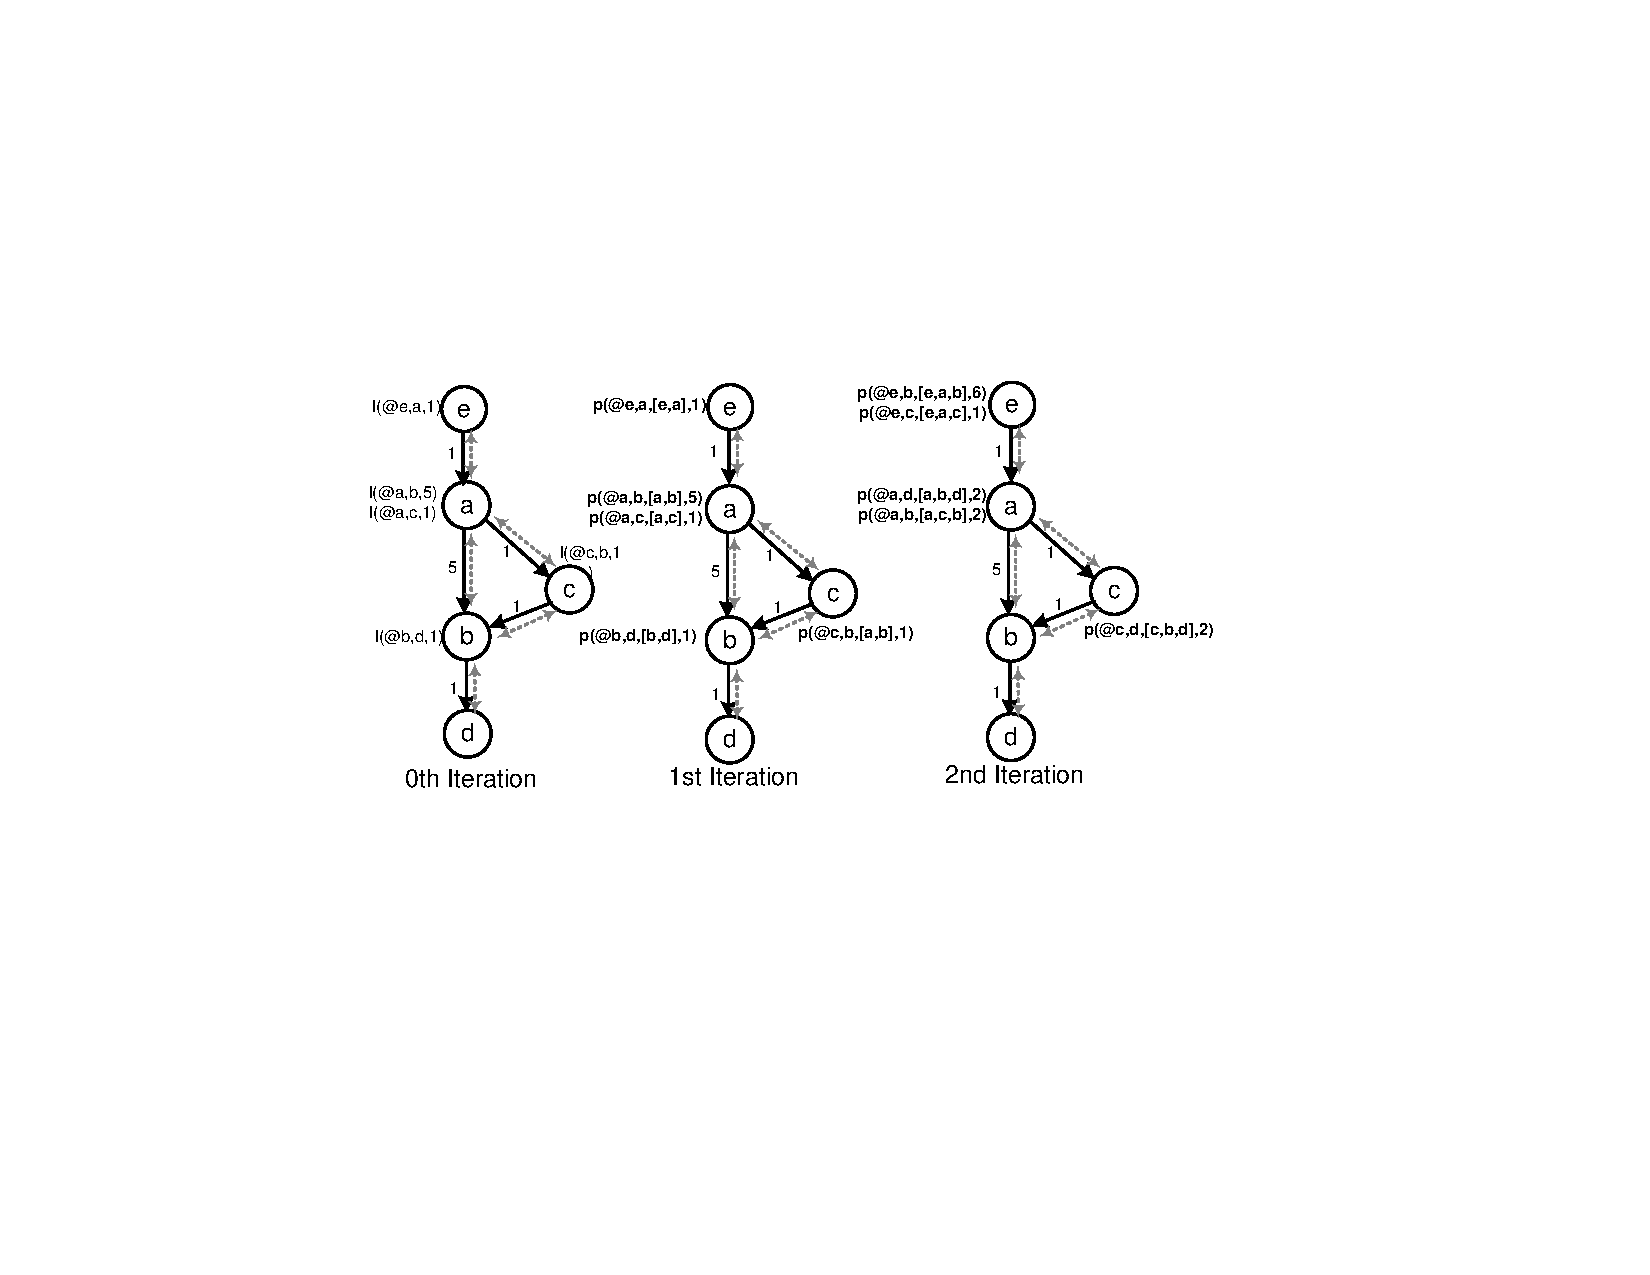
\includegraphics[width=3.5in]{graphs/example}
%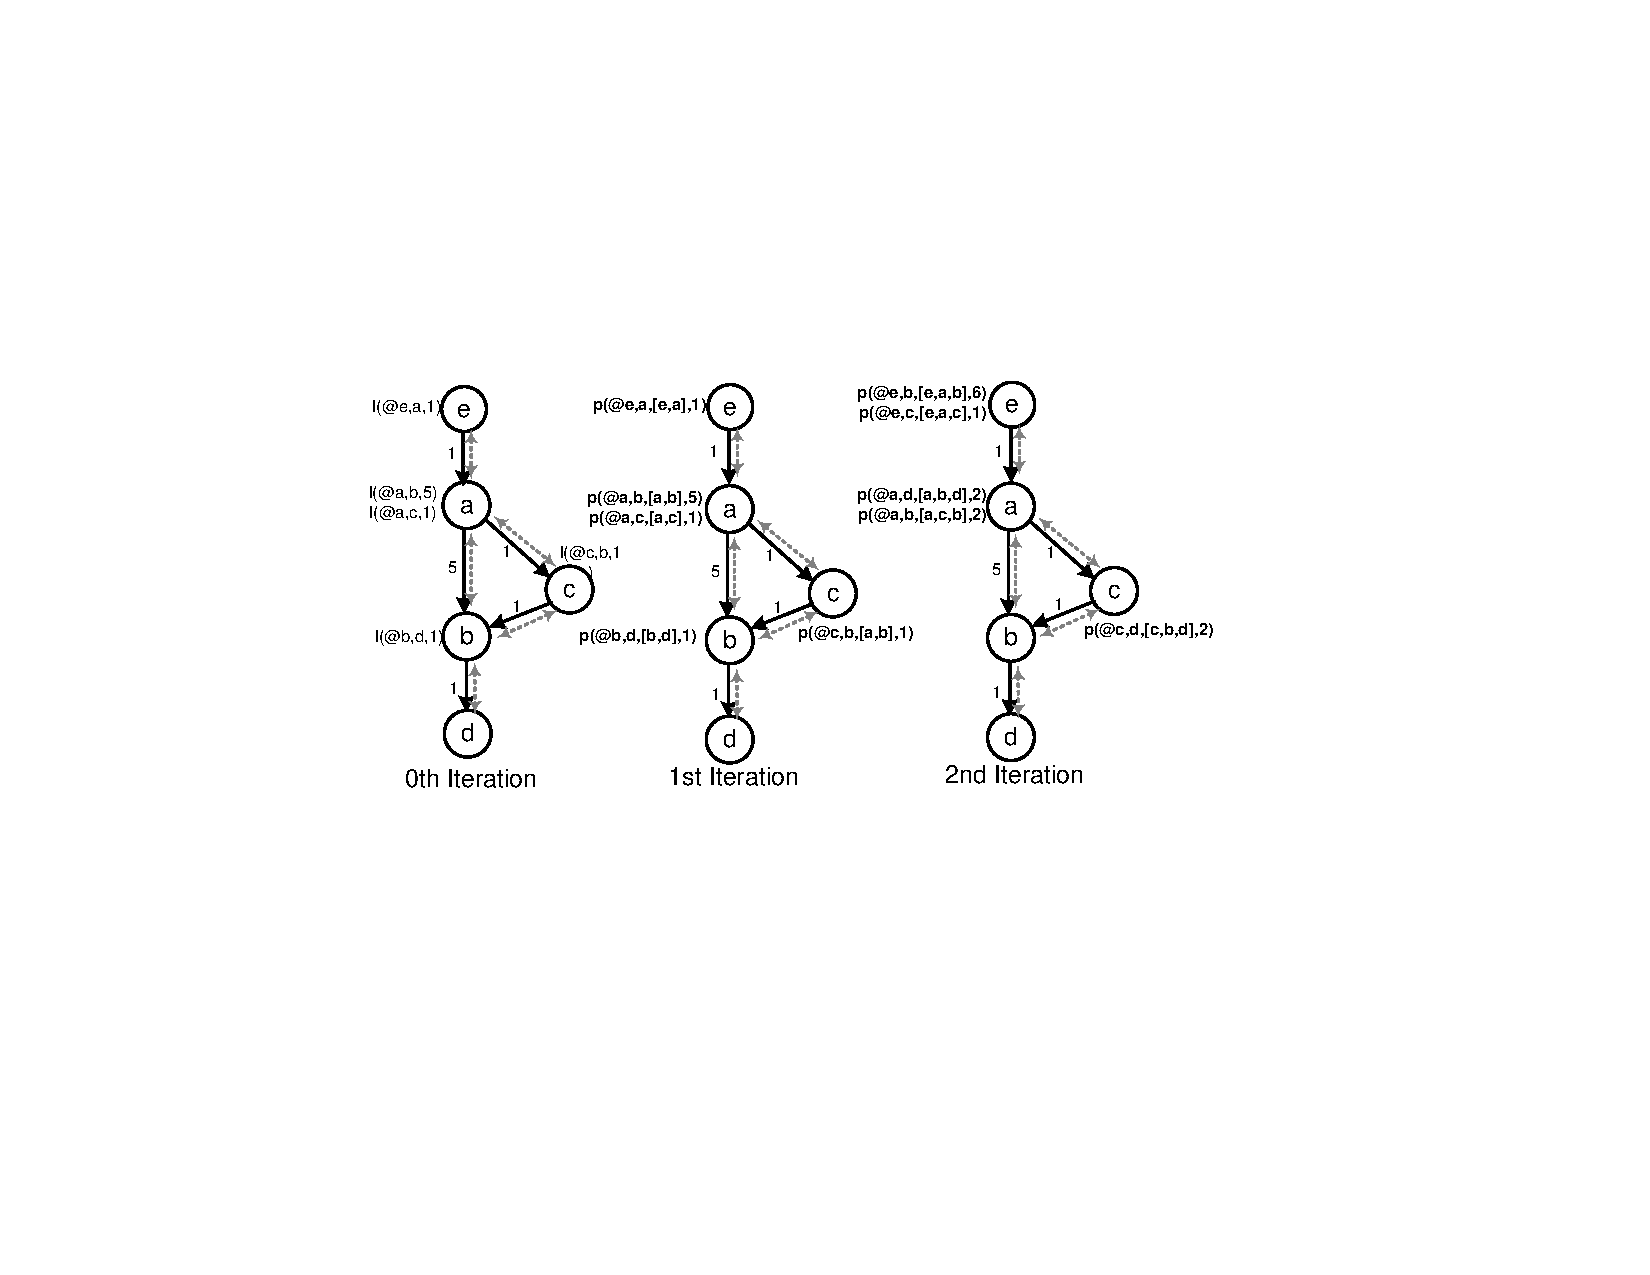
\epsfig{file=graphs/example., width=3.5in}
\caption{\label{SP example}{\small Nodes in the network are running
    the shortest-path query. We only show newly derived tuples at each
    iteration. For simplicity, we show only the derived paths along the
    solid lines even though the network connectivity is bidirectional
    (dashed lines).}}
\end{figure}                                              

For simplicity we will describe communication in {\em iterations}, where at each
iteration, each network node generates $paths$ of increasing hop
count, and then propagates these paths to neighbor nodes along
links. (We relax this notion in Section~\ref{sec:psn}.)  In the $1^{st}$ iteration, all nodes initialize their local
path tables to 1-hop paths using rule sp1. In the $2^{nd}$ iteration,
using rule sp2, each node takes the input paths generated in the
previous iteration, and computes 2-hop paths, which are then
propagated to its neighbors. For example, \nd{path(@a,d,[a,b,d],6)} is
generated at node {\em b} using \nd{path(@b,d,[b,d],1)} from the
$1^{st}$ iteration, and propagated to node {\em a}. In fact, many
network protocols propagate only the {\em nextHop} and avoid sending
the entire path vector.

%\jmh{Again, maybe we should leave out
%  nextHop?  Or instead say here that an alternative to passing paths
%  is to keep next-hops, which replaces the concat function with a
%  variable...?}

As paths are computed, the shortest one is incrementally
updated. For example, node $a$ uses rule sp1 to compute
\nd{path(@a,b,[a,b],5)}, and then sets its shortest path to
\nd{shortestPath(@a,b,[a,b],5)} using rule sp4. In the next iteration,
node $a$ receives \nd{path(@a,b,[a,c,b],2)} from node \nd{c} which has
lower cost compared to the previous shortest cost of 5, and hence
\nd{shortestPath(@a,b,[a,b],2)} replaces the previous tuple (the first
two fields of source and destination are the primary key of this relation).

Interestingly, while \Dlog is a language to describe networks, there
are no explicit communication primitives. All communication is
implicitly generated during rule execution as a result of data
placement specifications. For example, in rule \nd{sp2}, the \nd{path} and \nd{link}
predicates have different location specifiers, and in order to execute
the rule body of \nd{sp2} based on their matching fields, \nd{link}
and \nd{path} tuples have to be shipped in the network. It is the
movement of these tuples that will generate the messages for the
resulting network protocol.  


\subsection{Language Extensions}

We describe two extensions to the \Dlog language: {\em
  link-restricted rules} that limit the expressiveness of the
language in order to capture physical network constraints, and  
soft-state storage persistence commonly used in networking
protocols.

\subsubsection{Link-Restricted Rules}

In the above path vector protocol, the evaluation of a rule must
depend only on communication along the physical links.  In order to
send a message in a low-level network, there needs to be a link
between the sender and receiver. This is not a natural construct in
Datalog. Hence, to model physical networking components where
full connectivity is not available, \Dlog provides
restrictions ensuring that rule execution results in
communication only among nodes that are physically connected. This is
syntactically achieved with the use of the special \nd{link} predicate
in the form of {\em link-restricted rules}. A {\em link-restricted}
rule is either a local Datalog rule, or a rule with the following
properties:
\begin{myenumerate}
\item There is exactly one link predicate in the body
\item All other predicates (including the
      head predicate) have their
  location specifier set to either the first (source) or second
  (destination) field of the link predicate. 
\end{myenumerate}

This syntactic constraint precisely captures the requirement that we
be able to operate directly on a network whose link connectivity is
not a full mesh.  Further, as we demonstrate in
Section~\ref{sec:queryPro}, link-restriction also guarantees that all
programs with only link-restricted rules can be rewritten into a
canonical form where every rule body can be evaluated on a single
node, with communication to a head predicate along links. The following is an example of
a link-restricted rule:
\begin{NDlog}
p(@Dest,...) :- link(@Src,Dest...),p1(@Src,...),p2(@Src,...),
                ..., pn(@Src,...).
\end{NDlog}
The rule body of this example is executed at \nd{@Src} and the resulting $p$
tuples are sent to \nd{@Dest}, preserving the communication constraints along
links. Note that the body predicates of this example all have the same
location specifier: \nd{@Src}, the source of the link. In contrast, rule
\nd{sp2} of the \emph{shortest path} program is link-restricted but has some
relations whose location specifier is the source, and others whose
location specifier is the destination; this needs to be rewritten
to be executable in the network, a topic we return to in
  Section~\ref{subsec:ruleLocalization}. 
% While link-restricted rules
% limit the expressiveness of the permitted set of declarative networks,
% the restrictions enable us to better reason about eventual consistency
% of network protocols by placing constraints on FIFO link channels.
% \jmh{The material mentioned in the last
%   sentence is covered in \ref{subsec:ruleLocalization}, no?  Should we
%   try to move localization up here next to link restriction?  Seems
%   kind of natural.} \petros{I kind of like the current location of
%   localization. This is about language semantics. The localization section is
%   about query plan generation.}

Note that in a fully-connected network environment, an \Dlog parser can
be configured to bypass the requirement for link-restricted rules.


%See \cite{declareNetworks} for
%details.




%\reminder{Add a discussion on link-restricted rules. Proofs in SIGMOD paper}

\subsubsection{Soft-state Storage Model}
\label{sec:dn:softstate}

Many network protocols use the {\em soft-state}~\cite{clark88design}
approach to maintain distributed state. In the soft state storage
model, stored data have an associated {\em lifetime} or time-to-live
(TTL). A soft-state datum needs to be periodically refreshed; if more time
than a TTL passes without a datum being refreshed, that datum is deleted.  Soft
state is often favored in networking implementations because in a very
simple manner it provides well-defined eventual consistency
semantics. Intuitively, periodic refreshes to network state ensure
that the eventual values are obtained even if there are transient
errors such as reordered messages, node disconnection or link
failures.  However when persistent failures occur, no coordination is
required to register the failure: any data provided by failed nodes is
organically ``forgotten'' in the absence of refreshes.

We introduced soft-state into the \Overlog~\cite{declareOverlays}
declarative networking language, an extension of \Dlog. One additional
feature of \Overlog is the availability of a
\nd{materialized}~\cite{declareOverlays} keyword at the beginning of
each \Dlog program to specify the TTL of predicates. For example,
the definition \nd{materialized(link, \{1,2\}, 10)} specifies that the
\nd{link} table has its primary key set to the first and second
fields (denoted by \nd{\{1,2\}}),
% \footnote{Following the
  % conventions of the \Pitu declarative networking system, field 0
  % is reserved for the predicate name.} 
and each \nd{link} tuple has a
lifetime of 10 seconds.  If the TTL is set to infinity, the predicate
will be treated as {\em hard state}, i.e., a traditional relation that does not involve timeout-based deletion.

% \jmh{Hard state semantics are notably missing here.  I think you
%   should describe them w.r.t. local view materialization of Datalog.
%   You may also want to cite your thesis w.r.t, the subtleties of rules
%   that mix hard and soft state.  My group is still not sure how we
%   like to think about state updates for hard state, BTW.}

The \Overlog soft-state storage semantics are as
follows. When a tuple is derived, if there exists another tuple with
the same primary key but differences on other fields, an {\em update}
occurs, in which the new tuple replaces the previous one. On the other
hand, if the two tuples are identical, a {\em refresh} occurs, in
which the existing tuple is extended by its TTL.

If a given predicate has no associated \nd{materialize}
declaration, it is treated as an {\em event} predicate: a soft-state
predicate with TTL=0. Event predicates are transient tables, which are
used as input to rules but not stored. They are primarily used to
``trigger'' rules periodically or in response to network events. 
For example, utilizing \Overlog's
built-in \nd{periodic} event predicate, the following rule enables node \nd{X}
to generate a \nd{ping} event every 10 seconds to its neighbor \nd{Y}
denoted in the \nd{link(@X,Y)} predicate: 

\begin{NDlog}
ping(@Y,X) :- periodic(@X,10), link(@X,Y).
\end{NDlog}

Subtleties arise in the semantics of rules that mix event, soft-state
and hard-state predicates across the head and body.  One issue
involves the expiry of soft-state and event tuples, as compared to
deletion of hard-state tuples. In a traditional hard-state model,
deletions from a rule's body relations require revisions to the
derived head relation to maintain consistency of the rule.  This is
treated by research on materialized view
maintenance~\cite{rossMatviews}.  In a pure soft state model, the head
and body predicates can be left inconsistent with each other for a
time, until head predicates expire due to the lack of refreshes from
body predicates. Mixtures of the two models become more subtle.  We
provided one treatment of this issue~\cite{boonThesis}, which has
subsequently been revised with a slightly different interpretation
~\cite{evitaRaced}. There is still some debate about the desired
semantics, focusing around attempts to provide an intuitive
declarative representation while enabling familiar event-handler
design patterns used by protocol developers.

%and Navarro details the operational semantics
%embodied in a version of the P2 implementation~\cite{Navarro}. 


% 
% \jmh{Perhaps add a ``Discussion'' subsection that exposes some of the soft underbelly of our semantics.  One issue is that we allow ``hard-state'' tables in the heads of rules, whereas in  Datalog the heads are IDB tables (``views'').  IN some cases this is consistent with materialized view semantics (all hard state rules).  In others, it's more like ``insert'': we keep the tuples in those tables persistent even when the bodies don't support those tuples anymore (e.g. soft-state expiry, event tables).  Another issue: how do we model aggregation/negation w.r.t. delayed delivery of tuples?  There are more of these kinds of warts exposed in Navarro's paper on the ``operational semantics of declarative nets''.  }

\subsubsection{Additional Extensions of \Overlog}
\Overlog adds a number of features to \Dlog.  In addition to soft state, \Overlog adds support for negation and aggregation, including checks for stratification.  It also adds the ability to update the database via derivation of new facts to be inserted into database tables, as well as explicit deletion rules whose effects are deferred until after fixpoint.  \Overlog also provides a notion of unique keys for a relation, and the ability for the derivation of a new fact to ``overwrite'' a previous fact with a matching key.  State management and event handling semantics in \Overlog and related languages have been an evolving mix of declarative and operational notions~\cite{declareOverlays,dsn,navarro,evita,boom}, and are still a subject of active research.
